The Bluetooth stack has many layers. For this project the important layers are the HCI, LMP, and the physical layer(Bluetooth Radio). As seen in figure \ref{fig:bt_stack}. We have already discussed the LMP in a earlier section. The HCI and the physical layer will be discussed here below.

\begin{figure}
  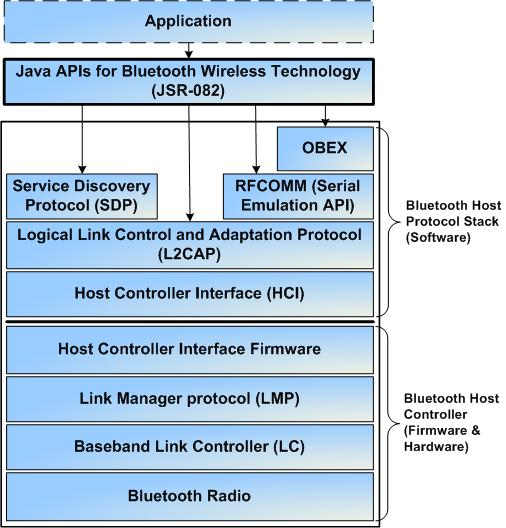
\includegraphics[scale=0.8]{images/bluetoothstack.jpg}
  \caption{The Bluetooth stack}
  \label{fig:bt_stack}
  \captionsetup{font={footnotesize,bf,it}}
  \caption*{\url{http://www.oracle.com/technetwork/testcontent/fig1-1-158000.jpg}}
\end{figure}

\subsubsection{Physical layer}
	% How we Gather data form the ubertooth
	In order to eavesdrop a Bluetooth communication we used the Ubertooth 1 tool presented above. This tool is able to decode packet from a targeted Bluetooth communication.
	The LAP(Lower Address Part) was known for the two devices. As explained in the literature review the Ubertooth tool retrieve the important parameters (UAP, clocks) used to sniff a connection thanks to that address. Once the tool was able to sniff and fallow a communication between the two devices it was possible for it to decode packets.
	In order to have relevant information the authors conducted experiments in a certain way. Indeed several captures have been performed recording:
\begin{itemize}
	\item[•] The pairing process between the two devices
	\item[•] The de-authentication process between two devices
	\item[•] The exchange of different data format (videos, pictures, notification) 
\end{itemize}
		 
\subsubsection{HCI layer}
	% How we Gather data form the hci
	Due to increasing use of Bluetooth; Android, since Android 4.4, have added a functionality available for developers to sniff Bluetooth packets at the HCI layer. This tool permits to monitor Bluetooth traffic in forms of pcaps logs for Wireshark. 
	The HCI layer is just above the LMP layer where authentication and encryption/encapsulation takes place. The data and messages exchanged at that layer are then in clear text and packets are not encapsulated. Then they are easily identifiable and easy to monitor.
	The experiments performed above at the RF layer have been performed in the same way (and at the same time) at the HCI layer. This as been done for analysis purposes.
	